% This is samplepaper.tex, a sample chapter demonstrating the
% LLNCS macro package for Springer Computer Science proceedings;
% Version 2.20 of 2017/10/04
%
\documentclass[runningheads]{llncs}
%
\usepackage{float}
\usepackage{graphicx}
% Used for displaying a sample figure. If possible, figure files should
% be included in EPS format.
%
% If you use the hyperref package, please uncomment the following line
% to display URLs in blue roman font according to Springer's eBook style:
% \renewcommand\UrlFont{\color{blue}\rmfamily}

\begin{document}
%
% \title{Optimizing Routes for Medicine Distribution \\Using Team Ant Colony System\thanks{Supported by organization x.}}
\title{Optimizing Routes for Medicine Distribution \\Using Team Ant Colony System}
%
\titlerunning{Optimizing Routes Using Global Optimizers}
% If the paper title is too long for the running head, you can set
% an abbreviated paper title here
%
% \author{First Author\inst{1}\orcidID{0000-1111-2222-3333} \and
% Second Author\inst{2,3}\orcidID{1111-2222-3333-4444} \and
% Third Author\inst{3}\orcidID{2222--3333-4444-5555}}
\author{Renan Costa Alencar\inst{1}\orcidID{0000-0003-0028-558X} \and \\
Clodomir J. Santana Jr.\inst{1}\orcidID{0000-0001-7869-7184}
\\
Carmelo J. A. Bastos-Filho\inst{1}\orcidID{0000-0002-0924-5341}}
%
\authorrunning{R. C. Alencar, C. J. Santana Jr. and C. J. A. Bastos-Filho}
% First names are abbreviated in the running head.
% If there are more than two authors, 'et al.' is used.
%
% \institute{Princeton University, Princeton NJ 08544, USA \and
% Springer Heidelberg, Tiergartenstr. 17, 69121 Heidelberg, Germany
% \email{lncs@springer.com}\\
% \url{http://www.springer.com/gp/computer-science/lncs} \and
% ABC Institute, Rupert-Karls-University Heidelberg, Heidelberg, Germany\\
% \email{\{abc,lncs\}@uni-heidelberg.de}}

\institute{Polytechnic University of Pernambuco, University of Pernambuco, Recife, Brazil\\
\email{\{rca2,cjsj,carmelofilho\}@ecomp.poli.br}}

%
\maketitle              % typeset the header of the contribution
%
\begin{abstract}
Distributing medicine using multiple deliverymen in big hospitals is considered complex and can be viewed as a Multiple Traveling Salesman Problem (MTSP). MTSP problems aim to minimize the total displacement of the salesmen, in which all intermediate nodes should be visited only once. The Team Ant Colony Optimization (TACO) can be used to solve this sort of problem. The goal is to find multiple routes with similar lengths to make the delivery process more efficient. Thus, we can map this objective in two different fitness functions: minimizing the longest route, aiming to be fair in the allocation of the workload to all deliverymen; and decreasing the total cost of routes, seeking to reduce the overall workload of the deliverymen. However, these objectives are conflicting. This work proposes the use of swarm optimizers to improve the performance of the TACO concerning these two objectives. The results using global optimizers for the parameters far outperformed the original TACO for the case study.

\keywords{Multiple Traveling Salesman Problem, \and Swarm Intelligence \and Hospital Logistics.}
\end{abstract}
%
%
%
\section{Introduction}
The Travelling Salesman Problem (TSP) and the Knapsack Problem (KP) are two of the most studied combinatorial optimization problems so far. TSP and KP belong to the set of NP-complete problems. In spite of the fact that they are tough to be solved even separately, there are some real-world problems that can be mapped as a combination of them, resulting in a complex task.
There is a TSP variation, which multiple salesmen engage in building a solution, the so-called Multiple Salesman Problem (MTSP). According to Bektas \cite{bektas2006multiple}, there is a variety of real-life problems, which are considered as MTSP, e.g., Routing Vehicle Problems (PRVs) with solution constraints. As stated in the MTSP definition, there are \(m > 1\) salesmen located initially in the same city which defines the depot. The other cities of the instance are defined as intermediate nodes. The MTSP aims to minimize the sum of route lengths with a constraint, which every route should begin and end at the depot node, and all intermediate nodes should visit only once. Besides, the MTSP problem has another constraint which there should be at least an intermediate node but the depot for each salesman route.
The KP is a combinatorial problem, which allocates space in a knapsack in advance according to an object selection. Hence, the total value of all chosen objects is maximized in the knapsack. Martello and Toth \cite{Martello:1990:KPA:98124} state that KP is a very often problem which appears in business, e.g., economic planning, and industry as cargo loading, cutting stock, and bin packing problems. They define the KP problem as an \(n\)-object vector of binary variables \(x_i\)(\(i=1,\ldots,n\)), in which the object \(i\) has a weight \(w_i\) and the knapsack has a capacity \(M\). If a fraction \(x_i\); \(0 \leq x_i \leq 1\), is placed in the knapsack, then a profit, \(g_i x_i\), is earned. The KP aims to find a combination of objects that maximizes the total profit from all chosen objects in the knapsack. While the knapsack's capacity is \(M\), the total weight of all chosen objects to be at most \(M\).

Although having those two problems associated is not unusual, they can appear in complex scenarios. For instance, the medicine distribution at big hospital centers can be viewed as an MTSP-KP instance. Both separation and distribution processes are seen as KP and MTSP instances, respectively. They have a high number of combinations and, even separated, those tasks are hard to be optimized, requiring sophisticated tools to tackle them. The hospital logistics can ensure patient's safety; however, it is one of the most challenging problems faced by hospital managers, especially in Brazil, due to meeting the organizational needs in a fast, accurate and efficient way. Furthermore, the financial resources addressed to hospital logistics should be implemented efficiently due to the low budget of Brazilian public hospitals.
Some approaches, based on mathematical methods and evolutionary algorithms, are used to optimize MTSP and KP instances. We can cite the following examples Genetic Algorithm – GA \cite{holland1992genetic}, Ant Colony Optimization - ACO \cite{dorigo2008particle} and Artificial Bee Colony - ABC \cite{karaboga2005idea}. These approaches aim to solve problems of steel production \cite{tang2000multiple}, cigarette distribution \cite{liu2009ant}, service orders \cite{barbosa2015aplicaccao}, sensor network routing \cite{wang2007hierarchical}, among others.

For the best of our knowledge, there are no reports in the literature regarding the use of global optimization processes to improve the performance of meta-heuristics deployed to solve the MTSP or MTSP-KP problem. Thus, there is still room for optimizing MTSP parameters with meta-heuristic algorithms aiming to achieve specific goals, especially when one needs to balance the length of the routes and the number of deliveries per agent simultaneously. Then, this work proposes a methodology to optimize MTSP parameters through global population-based optimizers, based on swarm intelligence based algorithms. We use the medicine distribution process with multiple routes as a case study.

The remainder of this paper is structured as follows. Section 2 introduces the basic concepts of some swarm intelligence-based algorithms to solve combinatorial problems. Section 3 describes the related works to the MTSP. Sections 4 and 5 depict the proposed model and the problem instance to be optimized. Section 6 outlines the scenarios and their settings to minimize the MTSP instance. Section 7 and 8 present the obtained results and the conclusions.

\section{Background}
\subsection{Team Ant Colony Optimization}
The Ant Colony Optimization (TACO), proposed by Vallivaara \cite{vallivaara2008team}, is based on the Ant Colony System (ACS) to solve MTSP instances. This basic generalization is made by replacing \(N\) ACS ants, which build solutions for TSP, with \(N\) teams of \(m\) members. An ant team represents a salesman in building the MTSP solution, and each team has its taboo list.

All ants of every team are placed at the depot at the beginning of the route construction. To distribute the workload, an ant $k$ with the shortest partial route chooses its next city $j$, at any moment of the building process, according to the Transition State Rule (TSR) equation, as shown in (\ref{eq:1}).

\begin{equation} \label{eq:1} 
    j = \Bigg\{
        \begin{tabular}{ll}
        argmax\(_{l \in J_k} \{\tau_{il}[\eta_{il}]^\beta\}\), & if $q \leq q_0$ \\
        J, & otherwise;
        \end{tabular}
\end{equation}

After choosing the next city, it is checked if another ant $l$ could add the chosen city to its route and end up with better total route length. If so, the ant $k$ can make its move first not choosing $j$. This checkpoint avoids the algorithm to force non-optimal solutions.

TACO has several parameters which are responsible for its behavior while building solutions. The initial probability  \(q_0\) determines whether the ants’ initialization has only deterministic or random choices (\(0 \leq q_0  \leq 1\)). The pheromone parameters \(\alpha\) and \(\beta\) define the weight of the pheromone trail and the visibility, respectively, in the choice of the next node by the ant. The parameter \(\xi\) controls the pheromone persistence when the Pheromone Update Rule (PUR) takes place locally, just after an ant moves from one city to another, that is, it includes one more edge on its route. Likewise, \(\rho\) regulates pheromone persistence for global PUR, i.e., at the end of each cycle of the algorithm.

\subsection{Particle Swarm Optimization}
Kennedy and Eberhart \cite{kennedy1999particle} proposed the Particle Swarm Optimization (PSO) method based on bird flocking. PSO is suitable for the optimization of continuous variables in a high-dimensional search space and presents high precision. It performs searching via a swarm of particles through an iteration process. Each particle moves towards its previous best (\(P_{best}\)) position and the global best (\(G_{best}\)) position in the swarm to achieve the optimal solution.

% \begin{equation} \label{eq:2}
%     _{i(t+1)} = x_{i(t)} + v_{i(t)}
% \end{equation}

The solution represents the particle position in the search space, a vector $x_i$. For each step, the particles have their positions according to their velocity vector $v_i$. The velocity clamping, an upper bound for the velocity parameter avoids particles flying out the search space. Likewise, the "constriction coefficient" strategy, proposed by Clerc and Kennedy \cite{clerc2002particle}, constricts the velocities through the dynamic swarm analysis.

% The inertia, in the Clerc’s constriction coefficient, represents the previous velocity, which provides the necessary momentum for particles to roam across the search space. On the other hand, the cognitive component in coefficient, determines the individual movement of each particle. It encourages the particles to moves towards their current best positions. Moreover, there is a "social" component within the constriction equation which implies the collaborative effect of the particles to find the optimal global solution.

% \begin{equation} \label{eq:3}
%     v_j = \omega v_j + c_1 r_1(P_{best} - x_j) + c_2 r_2(G_{best} - x_j)
% \end{equation} 

% \begin{equation} \label{eq:4}
%     v_{ij}(t+1) = \chi[v_{ij}(t+1) + \varphi_1(v_{ij}(t) - x_{ij}(t)) + \varphi_2(\hat{y}_{ij}(t) - x_{ij}(t))]
% \end{equation}
% where $\chi = \frac{2}{4 - \varphi - \sqrt{\varphi^2 - 4\varphi}}$, $\varphi = C_1 + C_2, \varphi_1 = c_1, \varphi_2 = c_2$

\subsection{Fish School Search}
Bastos-Filho et al. \cite{bastos2008novel} developed a population-based search algorithm inspired by fish swimming behavior, which expands and contracts while looking for food. The Fish School Search (FSS) algorithm considers the individual and collective fish movements. This optimization algorithm does not present the same exploitation capability of the PSO, but it has the capability to find good solutions in a search space with many local minima.
Each fish, in \(n\)-dimensional location, represents a feasible solution for the problem. Its success is measured by its weight, a cumulative account of how successful the search for each fish in the school has been. The fishes not only store information about their weight but also position in the search space.
FSS consists of moving and feeding operators. On the individual movement, each fish randomly moves towards a position in its neighborhood looking for promising regions. After moving to new positions, all fishes have their weights updated. The weight update is determined by the individual movement success, which is computed through the fitness of current and new positions. After feeding all fishes, the collective-instinctive movement takes place. All fishes move towards an influence vector. Those fishes that improved their fitness in the current iteration generate this vector.
At the end of the current iteration, the school contracts or expands according to the volitive-collective movement operator. The school's contraction results in an exploitation search whereas its expansion make the school explore the search area avoiding local minima. Thus, the volitive operator computes the school's barycenter. This last operator gives to the FSS the capability to self-adjust the granularity of the search along the optimization process.

% \begin{equation} \label{eq:5}
%     n_{ij} = x_{ij(t-1)} + step_{ind} \times random[-1,1]
% \end{equation}

% \begin{equation} \label{eq:6}
%     W_{i(t)} = W_{i(t-1)} + \frac{\Delta f_{i(t)}}{max[\Delta f_{i(t)}]}
% \end{equation}

% \begin{equation} \label{eq:7}
%     m_{j(t)} = \frac{\sum_{}^{} N_i = x_{ij(t)} \times W_{ij(t)}}{\sum_{}^{} N_i = W_{ij(t)}}
% \end{equation}

% \begin{equation} \label{eq:8}
%     x_{ij(t)} = x_{ij(t)} + m_{j(t)}
% \end{equation}

% \begin{equation} \label{eq:9}
%     B_j = \frac{\sum_{}^{} x_{ij(t)W_{ij(t)}}}{\sum_{}^{} W_{ij(t)}}
% \end{equation}

% \begin{equation} \label{eq:10}
%     x_{ij(t)} = x_{ij(t)} \pm step_{vol}\frac{x_{ij(t) - B_j}}{dist(x_{ij(t)}, B_j)}
% \end{equation}

\section{Related Works}
We did not find any approach related to medicine distribution until the present moment, but there is a set of computational problems, which are transversal to the tackled problem. Those problems have been studied to improve commercial production and distribution under one or more objective constraints.
Somhom, Modares and Enkawa \cite{somhom1999competition} use a Competition-Based Neural Network (CBNN) to minimize the longest route in an MTSP (based on the TSPLIB) instance with a single depot closed routes. Tang et al. \cite{tang2000multiple} use a Modified Genetic Algorithm (MGA) to improve production scheduling of hot rolling from an iron and steel industry in China. Carter and Ragsdale \cite{carter2006new} use a Genetic Algorithm (GA) with a new chromosome and MTSP operators. Wang et al. \cite{wang2007hierarchical} use the Ant Colony System (ACS) to group and route sensor nodes from a wireless multimedia network with a limited time interval as a constraint. Vallivaara \cite{vallivaara2008team} proposes the Team Ant Colony Optimization, based on ACS rules to manage routes with multiple robots in a hospital environment. The problem constraint is to minimize the longest route and the sum of routes. Liu et al. \cite{liu2009ant} use the ACS and the Max-Min Ant System to solve the distribution of cigarettes in a Chinese company. Barbosa and Kashiwabara \cite{barbosa2015aplicaccao} use the Single Team Ant Colony System (STACS), based on TACO, to route the service orders in an energy distribution company.

\section{Proposed Model}
The proposed model consists of using a base algorithm to compute the best solutions for an MTSP instance while having a global optimizer algorithm to seek the best parameters sets for the base algorithm. In this work, we deploy the Team Ant Colony Optimization (TACO) as the base algorithm. Moreover, the Particle Swarm Optimization (PSO) and the Fish School Search take part in the optimization of the values for TACO parameters.

\begin{figure}
  beac   \centering
    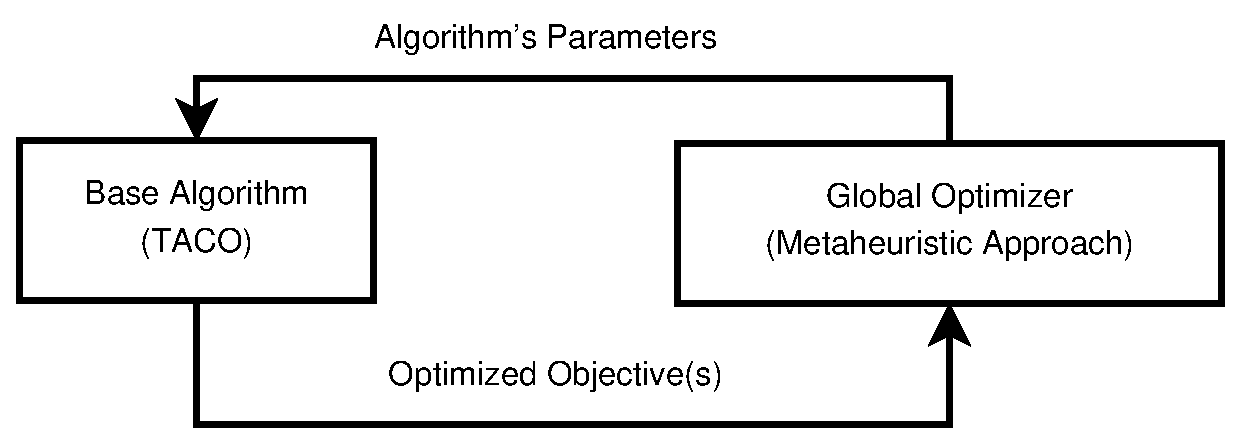
\includegraphics[width=0.5\textwidth]{Diagram1.eps}
    \caption{Proposed Model for optimizing the TACO} \label{fig:1}
\end{figure}

As shown in Figure \ref{fig:1}, the Global Optimizer (GO) starts to generate a set of values for the TACO’s parameters. In this case, the optimized parameters from TACO are $\alpha$ (pheromone relevance), $\beta$ (relevance of pheromone’s visibility), $\xi$ (pheromone persistence, local update) and $\rho$ (pheromone persistence, global update). Then, TACO builds a set of best solutions based on the optimized parameters. Next, TACO returns to GO the set of best solutions, which are evaluated to the meta-heuristic algorithm. As the iterations happen, the GO keeps a record of the best set of parameters, which has been found so far. The execution finishes when the GO reaches the limit of iterations.

\section{Problem Instance}
A Medicine Distribution Center (MDC) at a public hospital in Brazil usually executes the orders manually, both packaging the orders and building the routes. It does not matter how long it would take for the deliverymen to do that. Due to the considerable time variation for answering the orders, it is difficult to determine the delivery capacity for each agent to minimize individual costs of the built routes.

That real-world problem highlights a set of objectives, which can be optimized. One of those objectives is to reduce the total sum of the routes without worrying about the work balance between the deliverymen. Another objective is to have balanced routes at the end of order execution, which also results in more orders being executed at the same time interval, i.e., in this case, the target is to avoid a partially inoperative deliveryman because it has a route significantly shorter than the others.

Figure \ref{fig:2} highlights 16 pharmacies and an MDC, represented as \(V1\),  of a real hospital environment from Brazil represented as a graph with costs associated with distances for the deliveries. The MDC is the depot where the deliverymen start and finish their routes. A matrix, called cost matrix, contains the data of each pharmacy like identification (ID), latitude, longitude and its distance. The matrix helps to calculate the route cost. It is important to highlight that this graph shows the topology to reach the pharmacies, but do not explicit represent the geographical position.

\begin{figure}
    \centering
    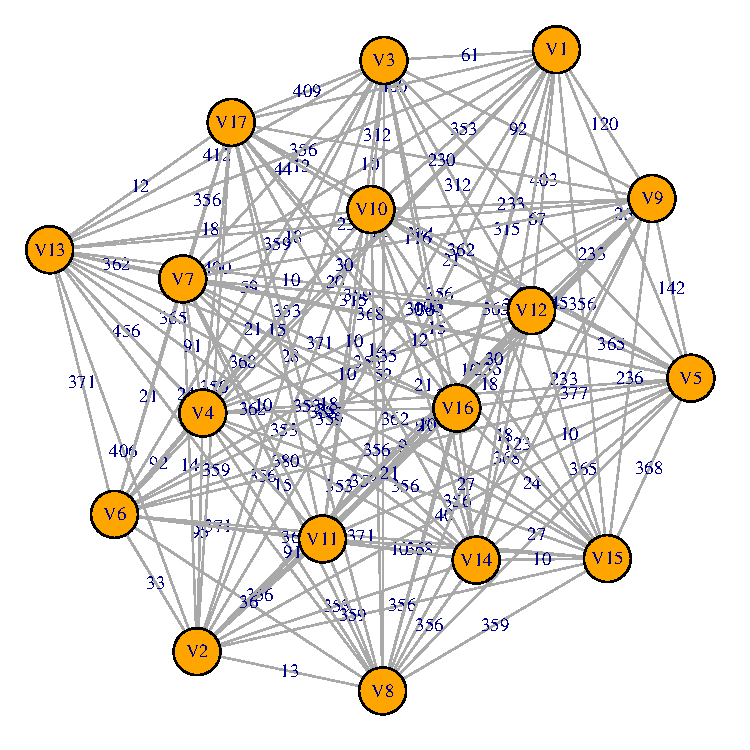
\includegraphics[width=0.45\textwidth]{Rplots.eps}
    \caption{Graph Model} \label{fig:2}
\end{figure}

Likewise, another matrix, called the data matrix, contains the delivery orders for each node in the built model. Each order includes IDs of deliveryman and pharmacy, the initial and final distances when the deliveryman left the MDC and the duration of the order. The data matrix helps to simulate a day of ordering in the depot. Also, there are four deliverymen to deliver the requests to the pharmacies.

As stated in Section 4, a global optimizer, based on swarm intelligence, is also used to improve the TACO results by optimizing its parameters. FSS and PSO are taken as a global optimizer of the TACO parameters. We assessed the PSO because of its capacity to refine the values for the parameters (good exploitation capability) and the FSS because of its capacity to escape from local optima during the optimization process. The standard values for the set of used parameters are: number of deliverymen \(M = 4\), the number of teams \(N = 10\), initial probability  \(q_0 = 0.5\), pheromone relevance \(\alpha = 0 .5\), visibility relevance \(\beta = 1.0\), pheromone persistence for local update \(\xi = 0.1\), pheromone persistence for global update \(\rho = 0.1\). A parameter test obtained those default values. The stop criterion is 1000 iterations for each independent run. The global optimizers optimize the subset of parameters \(P = \{\alpha,\beta,\xi,\rho\}\) in a range \(0 \leq P \leq 2\).

\section{Experimental setup}
The experiments presented in this section aims to show the effectiveness of the developed methodology applied to the real problem. In the first scenario, the algorithms are configured to minimize the total cost of the solutions, without considering the distribution of the workload between the teams, as in the general description of the MTSP. In the second scenario, the algorithms minimize the cost of the largest individual route of the solutions, aiming the construction of solutions formed by routes with equal costs among the deliverymen, as in the MTSP with workload balance.

All experiments were executed on a MacBook Pro (13-inch, Late 2011) with 2.4GHz Intel Core i5 CPU, 16GB of RAM (1333MHz DDR3) and macOS High Sierra (version 10.13.4) operating system. We used the database presented in Section 4. Then, we performed 30 independent runs of the algorithms for each experiment. TACO algorithm was coded in Java based on the proposed algorithm by Vallivaara \cite{vallivaara2008team}. The FSS is based on Bastos-Filho et al. \cite{bastos2008novel} version. The single objective PSO were taken from the jMetal framework \cite{durillo2011jmetal}.

TACO takes part in the experiment as a base algorithm. Before starting the experiments of the proposed model, a base test has to be taken to prove the effectiveness and robustness of the chosen algorithm. The default values for both scenarios are stated in Section 5. The FSS as a GO is executed with a stop criterion of 1000 iterations per run, and it has 30 independent runs. The values of FSS parameters were taken from \cite{bastos2008novel}. Similarly, the PSO has the same values of stop criterion and independent runs. The values of PSO parameter remained the same as in \cite{durillo2011jmetal}.

\section{Results}
The first set of experiments was carried out to minimize the Total Cost of Routes (TCR), i.e., the sum of each team's route. By comparing the results, the solution, which has the lowest total cost, is considered the best one. This scenario can be applied to real life when we aim to reduce the total amount of the deliverymen routes instead of prioritizing the work balance.

The second set of experiments aimed to minimize the Longest Route (LR) of the solutions keeping the same values of the parameters in the first scenario. That case is suitable for real situations when we prioritize the balance among the individual routes (work balance) rather than the total sum of routes.

\subsection{Experiments without Global Optimizers}
Table \ref{tab:1} shows the average execution time of the algorithm for each case. We obtained this value from the average of the time spent to execute the 1000 iterations with 30 independent runs of the algorithm, for one working day.

\begin{table}
    \centering
    \caption{Comparison of the Results with Average of 30 Independent Runs} \label{tab:1}
    \begin{tabular}{|c|c|c|c|c|c|c|c|c|}
        \hline
        \textbf{Approach} & \multicolumn{4}{|c|}{\textbf{Minimizing TCR}} & \multicolumn{4}{|c|}{\textbf{Minimizing LR}}\\
        \hline
        {} & TCR & S.D. & LR & S.D. & TCR & S.D. & LR & S.D.\\
        \hline
        TACO & 1.8 & 0.25 & 0.721 & 0.003 & 1.223 & 0.050 & 0.756 & 0.012\\
        \hline
        FSS	& 1.0797 & 0.002 & 0.747 & 0 & 1.944 & 0.335 & 0.719 & 0.001\\
        \hline
        PSO	& 1.115 & 0.032 & 0.750 & 0.003 & 2.048 & 0.333 & 0.720 & 0.005\\
        \hline
    \end{tabular}
\end{table}

TACO presented satisfactory results for the two MTSP variations: minimizing the total cost of the solution and minimizing the cost of the largest individual solution route (Table \ref{tab:1}). The small values of the standard deviations in the two tables confirm the robustness of the algorithm when generating solutions with costs close to the average of the 30 executions. Although LR is being minimized, TCR varies throughout the iterations. The same situation happens when TACO minimizes TCR. Bearing this in mind, there is still room to make improvements in the results of both objectives.


% \begin{figure}
%     \centering 
%     \begin{minipage}{.7\textwidth}
%         \includegraphics[width=\textwidth]{convergence-totalcost.eps}
%     \end{minipage}
%     \begin{minipage}{.7\textwidth}
%         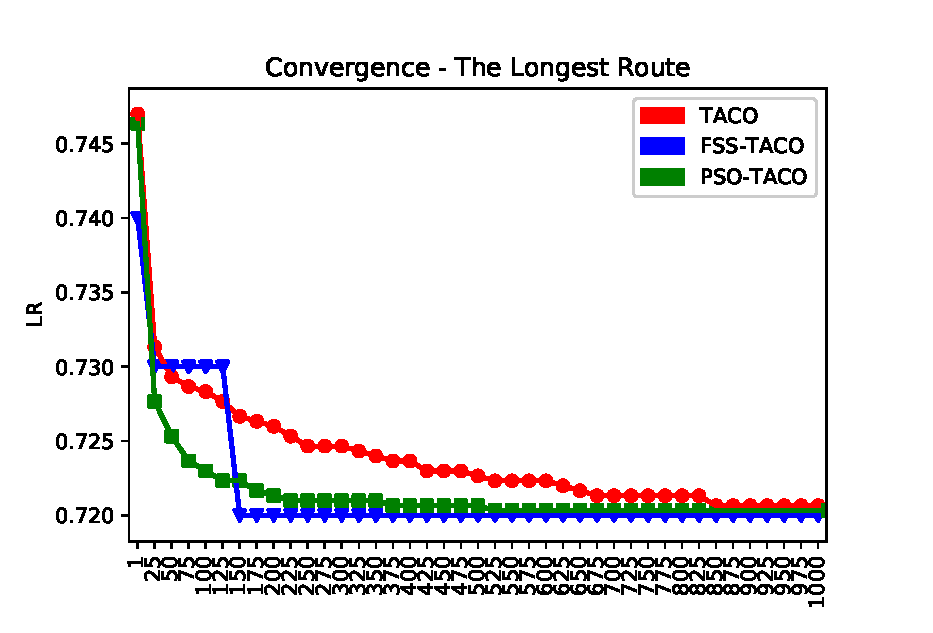
\includegraphics[width=\textwidth]{convergence-maxcost.eps}
%     \end{minipage}
%     \caption{Comparison among the three approaches when minimizing TCR and LR} \label{fig:3}
% \end{figure}


\subsection{Experiments with Global Optimizers}
The experiments carried out with global optimizer showed better results for both scenarios, as displayed in Table \ref{tab:1}. the approach having FSS as a GO (FSS-TACO) presented a better improvement when minimizing the longest route in comparison to the base algorithm. This result is due to the capability of the FSS-TACO to explore the search space. FSS-TACO has a lower standard deviation which corroborates to its robustness.

The approach having PSO as a GO (PSO-TACO) also had better results comparing to the TACO approach without global optimizers (see Table \ref{tab:1}). Its standard deviation also shows the robustness and effectiveness when optimizing TCR and LR.
\begin{figure}
    \centering
    \includegraphics[width=\textwidth]{convergence-unique.eps}
    \caption{Comparison among the three approaches when minimizing TCR and LR} \label{fig:3}
\end{figure}

\subsection{Comparison}
All the previous results are compiled in Table \ref{tab:1} for a better understanding of them. Comparing the three approaches, FSS-TACO got better results when minimizing both TCR and LR. It also had the lowest result with a standard deviation close to zero. As seen in Figure \ref{fig:3}, in both scenarios, FSS-TACO converged earlier than PSO-TACO and the base-algorithm. Results of PSO-TACO were also better than base-algorithm results and converged earlier than TACO as expected. 

Figure \ref{fig:4} shows the boxplots for both TCR and LR. When minimizing the TCR, we can notice that the results for the FSS-TACO far outperformed the others, and PSO-TACO varies more than TACO. When minimizing the LR, both FSS-TACO and PSO-TACO approaches outperformed TACO.
\begin{figure}
    \centering
    \includegraphics[width=\textwidth]{boxplot-unique.eps}
    \caption{Boxplots for TCR and LR considering TACO, FSS-TACO and PSO-TACO.} \label{fig:4}
\end{figure}

% \begin{figure}
%     \centering 
%     \begin{minipage}{.7\textwidth}
%         \includegraphics[width=\textwidth]{boxplot-totalcost.eps}
%     \end{minipage}
%     \begin{minipage}{.7\textwidth}
%         \includegraphics[width=\textwidth]{boxplot-maxcost.eps}
%     \end{minipage}
%     \caption{Standard Deviation of TCR and LR minimizations} \label{fig:4}
% \end{figure}

\section{Conclusions}
The proposed model described was efficient in the distribution of work orders among the deliverymen and in the creation of optimized routes to carry out the services. However, some questions need to be analyzed, such as multi-objective optimization of the total cost of the routes and the longest route and optimization of the deliverymen’s knapsacks.
For the creation of solutions optimized for MTSP in this work, an algorithm based on the ACO metaheuristic was implemented and associated with a global optimizer. The FSS and PSO were responsible for optimizing the TACO parameters to improve the results.
As shown in Section 6, FSS-TAO achieved the best results for both scenarios with the lowest minimization results for the Total Cost of Routes (TCR) and the Longest Route (LR) with standard deviations around zero. In those two cases, FSS-TACO as a global optimizer converged earlier than the other two approaches.

Another possible approach to the MTSP problem is to optimize both objectives simultaneously, TCR and LR. To achieve this goal, we aim to use a multi-objective optimization algorithm called Multi-Objective Fish School Search (MOFSS) as a globl optimizer for TACO's parameters.

% \paragraph{Sample Heading (Fourth Level)}
% The contribution should contain no more than four levels of
% headings. Table~\ref{tab1} gives a summary of all heading levels.

% begin{table}
% \caption{Table captions should be placed above the
% tables.}\label{tab1}
% \begin{tabular}{|l|l|l|}
% \hline
% Heading level &  Example & Font size and style\\
% \hline
% Title (centered) &  {\Large\bfseries Lecture Notes} & 14 point, bold\\
% 1st-level heading &  {\large\bfseries 1 Introduction} & 12 point, bold\\
% 2nd-level heading & {\bfseries 2.1 Printing Area} & 10 point, bold\\
% 3rd-level heading & {\bfseries Run-in Heading in Bold.} Text follows & 10 point, bold\\
% 4th-level heading & {\itshape Lowest Level Heading.} Text follows & 10 point, italic\\
% \hline
% \end{tabular}
% \end{table}


% \noindent Displayed equations are centered and set on a separate
% line.
% \begin{equation}
% x + y = z
% \end{equation}
% Please try to avoid rasterized images for line-art diagrams and
% schemas. Whenever possible, use vector graphics instead (see
% Fig.~\ref{fig1}).

% \begin{figure}
% \includegraphics[width=\textwidth]{fig1.eps}
% \caption{A figure caption is always placed below the illustration.
% Please note that short captions are centered, while long ones are
% justified by the macro package automatically.} \label{fig1}
% \end{figure}

% \begin{theorem}
% This is a sample theorem. The run-in heading is set in bold, while
% the following text appears in italics. Definitions, lemmas,
% propositions, and corollaries are styled the same way.
% \end{theorem}

%
% the environments 'definition', 'lemma', 'proposition', 'corollary',
% 'remark', and 'example' are defined in the LLNCS documentclass as well.
%

% \begin{proof}
% Proofs, examples, and remarks have the initial word in italics,
% while the following text appears in normal font.
% \end{proof}

% For citations of references, we prefer the use of square brackets
% and consecutive numbers. Citations using labels or the author/year
% convention are also acceptable. The following bibliography provides
% a sample reference list with entries for journal
% articles~\cite{ref_article1}, an LNCS chapter~\cite{ref_lncs1}, a
% book~\cite{ref_book1}, proceedings without editors~\cite{ref_proc1},
% and a homepage~\cite{ref_url1}. Multiple citations are grouped
% \cite{ref_article1,ref_lncs1,ref_book1},
% \cite{ref_article1,ref_book1,ref_proc1,ref_url1}.
%
% ---- Bibliography ----
%
% BibTeX users should specify bibliography style 'splncs04'.
% References will then be sorted and formatted in the correct style.
%
\bibliographystyle{splncs04}
\bibliography{reference}
%
% \begin{thebibliography}{8}
% \bibitem{ref_article1}
% Author, F.: Article title. Journal \textbf{2}(5), 99--110 (2016)

% \bibitem{ref_lncs1}
% Author, F., Author, S.: Title of a proceedings paper. In: Editor,
% F., Editor, S. (eds.) CONFERENCE 2016, LNCS, vol. 9999, pp. 1--13.
% Springer, Heidelberg (2016). \doi{10.10007/1234567890}

% \bibitem{ref_book1}
% Author, F., Author, S., Author, T.: Book title. 2nd edn. Publisher,
% Location (1999)

% \bibitem{ref_proc1}
% Author, A.-B.: Contribution title. In: 9th International Proceedings
% on Proceedings, pp. 1--2. Publisher, Location (2010)

% \bibitem{ref_url1}
% LNCS Homepage, \url{http://www.springer.com/lncs}. Last accessed 4
% Oct 2017


% \end{thebibliography}
\end{document}